\section{Base di dati sistema anagrafe}

\subsection{Abstract}

L'obiettivo è sviluppare un servizio che tenga ordinati e renda sempre disponibili tutte le informazioni relative a nomi, gruppi, peculiarità di ognuno dei sensori, delle aree, e dei lampioni. 

Queste informazioni sono particolarmente utili per contestualizzare ognuna delle componenti {\it{hardware}} del sistema.

\subsection{Analisi dei requisiti}

\subsection{Progettazione concettuale}

\subsection{Progettazione logica}

\subsubsection{Eliminazione delle generalizzazioni}

\paragraph{Misuratore}

Per evitare di accorpare le entità Sensore e Lampione nell'entità padre Misuratore, creando così dei campi NULL, è stato deciso di risolvere la generalizzazione mantenendo le tre entità inserendo le relazioni tra le entità figlie e l'entità padre.

\subsubsection{Modifiche, aggiunte e chiarimenti alle chiavi}

Tutte le chiavi primarie sono definite utilizzando le chiavi della progettazione concettuale, tranne nei seguenti casi.

\paragraph{Sensore} Diventando il Sensore un'entità a sé stante, vengono aggiunte una chiave primaria ed una chiave esterna che indica il Misuratore a cui fa riferimento.

\paragraph{Lampione} Diventando il Lampione un'entità a sé stante, vengono aggiunte una chiave primaria ed una chiave esterna che indica il Misuratore a cui fa riferimento.

\subsubsection{Schema concettuale ristrutturato - Schema Logico}

\begin{center}
    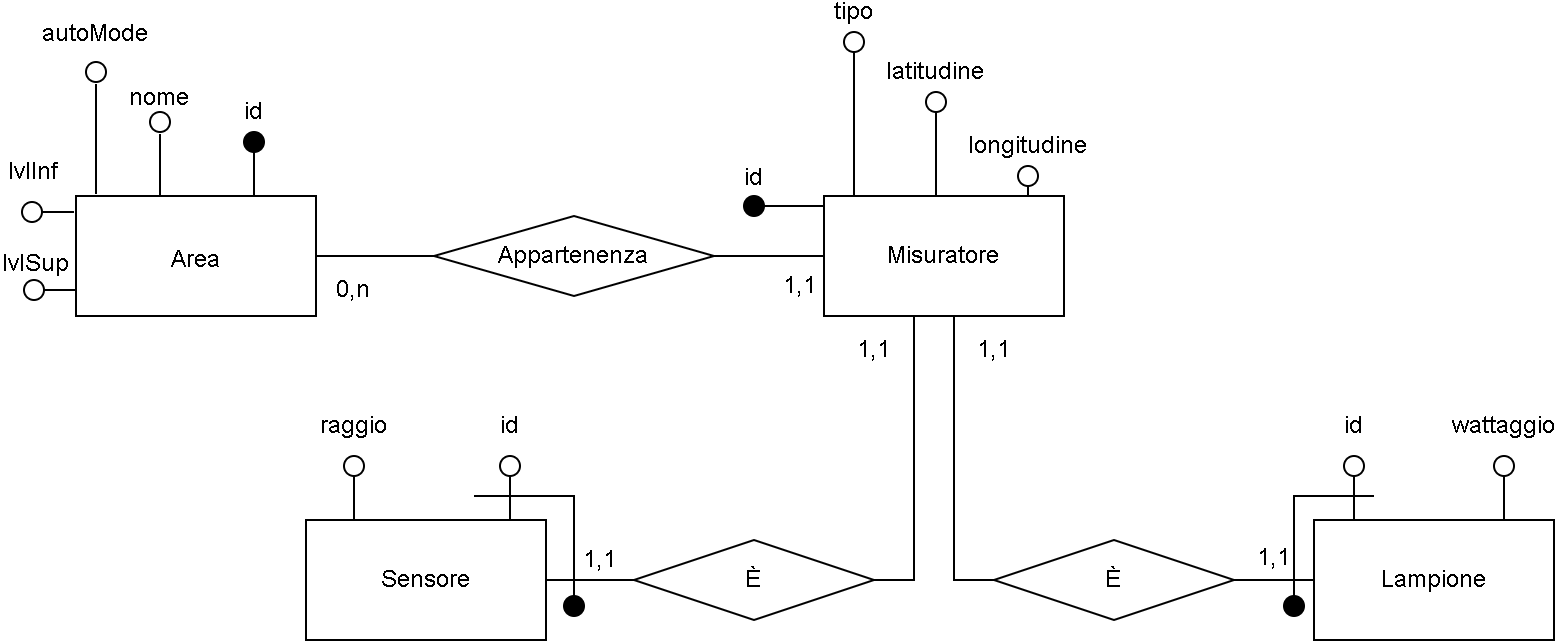
\includegraphics[width=12cm]{contenuti/specifica-basi-dati/img-sbd/anagrafica_logico.png}
\end{center}

\subsubsection{Descrizione schema relazionale}

Per questione di compatibilità con il DBMS alcuni nomi di attributi entità e relazioni sono stati normalizzati, utilizzando il camelCase, togliendo gli accenti, accorciando i nomi molto lunghi e con altre piccole accortezze.
La chiave primaria è indicata in \textbf{grassetto}, le chiavi esterne sono indicate con la \underline{sottolineatura}.

\textit{Area}(\textbf{id}, nome, autoMode, lvlInf, lvlSup) \\
\textit{Misuratore}(\textbf{id}, \underline{idArea}, tipo, latitudine, longitudine) \\
\textit{Sensore}(\textbf{id}, \underline{idMisuratore}, raggio) \\
\textit{Lampione}(\textbf{id}, \underline{idMisuratore}, luminosita)

\subsubsection{Vincoli di integrità referenziali}

\textbf{Sensore}.idMisuratore -> \textit{Misuratore}.id \\
\textbf{Lampione}.idMisuratore -> \textit{Misuratore}.id

\subsubsection{Check e constraint}

\paragraph{Area} In \textbf{Area} è attivato un check che controlla che il valore del livello inferiore sia sempre minore del valore del livello superiore.